\documentclass[en]{../../../../../../eplexam}

\usepackage{wrapfig}
\usepackage{enumitem}
\usepackage{gensymb}
\usepackage{graphicx}

\hypertitle{meca-FSAB1201}{1}{EPL}{1201}{2016}{Août}{All}
{Nathan Jacques \and Arthur van Stratum}
{Roland Keunings}


%\usepackage{soulutf8}
%\usepackage{amsmath}
%\usepackage{amssymb}
%\usepackage{mathrsfs}

\paragraph{Question 1}
Une poutre horizontale uniforme pesant 150N est mise en charge comme indiqué sur la figure. Calculez \phantom{blablablayjutfiytcdkiy,jjjjjjjj}
\begin{wrapfigure}[4]{l}{4cm}
	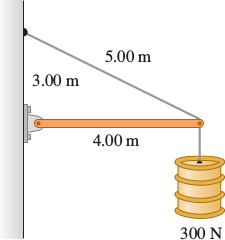
\includegraphics[width=4cm]{poutre}
\end{wrapfigure}
\begin{enumerate}[label=\alph*]
	\item la tension dans le câble incliné;
	\item les composantes horizontales et verticales de la force exercée par le mur sur la poutre.
\end{enumerate}
\vspace{3cm}

\paragraph*{Solution}

Voici le Free Body Diagram de la poutre (figure~\ref{fbd}). $H_v$ et $H_h$ sont les composantes verticales et horizontales de la force exercée par la poutre sur le mur. Comme la poutre est uniforme, son centre de masse se situe au milieu de celle-ci. En outre, on a, par les règles de trigonométries dans le triangle rectangle, $\cos \theta = 0.8$ et $\sin \theta = 0.6$ 

\begin{enumerate}[label=\alph*.]
	\item En calculant la somme des torques au point de contact entre le mur et la poutre,  on obtient facilement: $-2w-4w_{load}+4T \sin\theta = 0$ et donc, en isolant $T$, 
		\[\boxed{T = \frac{(150 \mathrm N)(2\mathrm m)+(300\mathrm N)(4\mathrm m)}{(4\mathrm m)(0.6)} = 625\mathrm N}\]
	\item \[\sum F_x = H_h-T -\cos \theta = 0 \implies H_h = (625\mathrm N)(0.8) = \boxed{500\mathrm N}\]

		\[\sum F_y = H_v-w-w_{load}+T\sin \theta = 0 \implies H_v = 150\mathrm N + 300\mathrm N - (625\mathrm N)(0.6) = \boxed{75\mathrm N}\]
\end{enumerate}

\begin{figure}[h!]
	\center
	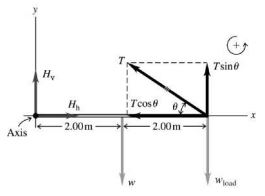
\includegraphics[width=4cm]{FBD1}
	\caption{Free body diagram}
	\label{fbd}
\end{figure}


\newpage

\paragraph{Question 2}
Une perle peut glisser sans frottement le long d'un anneau circulaire de rayon 0,1 m. L'anneau est en rotation autour d'un diamètre vertical
à une vitesse constante de 4 tours par seconde. \phantom{qsdfghjkljdsfgyhjkdrftghj}
\begin{wrapfigure}[3]{l}{4cm}
	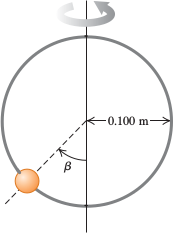
\includegraphics[width=4cm]{cercle}
\end{wrapfigure}
\begin{enumerate}[label=\alph*.]
	\item calculez l'angle $\beta$ auquel la perle est en équilibre vertical;
	\item la perle peut-elle atteindre un angle de 90\degree? Motivez votre réponse;
	\item Que se passe t'il si l'anneau tourne à 1 tour par seconde.
\end{enumerate}

\vspace{3cm}

\paragraph*{Solution}

Commençons par mettre de l'ordre dans les données et établir quelques relations utiles à la résolution de l'exercice.
Lorsque l'anneau tourne autour de son axe, la perle se déplace sur un cercle de rayon $R = r \sin \beta$ et nous savons que la force exercée sur la perle est orientée radialement.

\begin{figure}[!h]
	\centering
		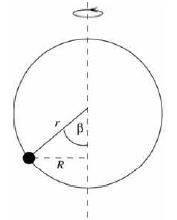
\includegraphics[width=4cm]{bead}
	\quad
		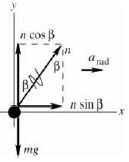
\includegraphics[width=4cm]{FBD2}
	\caption{Perle}
\end{figure}

Grâce au Free Body Diagram, appliquons le second principe de Newton $\displaystyle{\sum \vec{F} = m\vec{a}}$,
\[\sum F_y = n \cos \beta - mg = 0 \iff n = \frac{mg}{\cos \beta}\]
\[\sum F_x = n \sin \beta= ma_{rad} \iff n = \frac{ma_{rad}}{n \sin \beta}\]

En égalant les deux expressions de $n$ ainsi trouvées, on a

\begin{align}
	\left( \frac{mg}{\cos \beta}\right) \sin \beta & =  ma_{rad} \nonumber \\
	\tan \beta & =  \frac{a_{rad}}{g}
	\label{eq1}
\end{align}

Pour $a_{rad}$, on sait que $a_{rad}=\frac{v^2}{R}$ et que $v = \frac{2\pi R}{T}$ ce qui implique que $a_{rad} = \frac{4\pi^2 R}{T^2}$ où $T$ est la période de rotation de l'anneau. Or, comme $R = r \sin \beta$, $a_{rad} = \frac{4\pi^2 r \sin \beta}{T^2}$
Ce qui nous donne, en remplaçant dans \ref{eq1},
\[\tan \beta = \frac{4\pi^2 r \sin \beta}{T^2 g}\]

Si $\beta = 0 \implies \sin \beta = 0$, l'équation est satisfaite et sinon, $\forall \beta \in \left]0,\frac{\pi}{2}\right[$, on peut simplifier de chaque côté par $\sin \beta$
\[\cos \beta = \frac{T^2g}{4\pi^2r}\]

\begin{enumerate}[label=\alph*.]
	\item Pour 4 tours/seconde, la période $T = 0.25 \mathrm s$. On a donc \[\cos \beta = \frac{(0.25\mathrm s)^2(9.8\mathrm{\frac{m}{s^2}})}{4\pi^2(0.1 \mathrm m)} \implies \boxed{\beta = 81.1\degree}\]
	\item $\beta = 90\degree \implies \cos \beta = 0$ or cela n'arrivera que si $T=0$ ce qui est impossible car cela demande une vitesse de rotation infinie.
	\item Pour 1 tour/seconde, la période $T = 1 \mathrm s$. On a donc $\displaystyle{\cos \beta = \frac{(1\mathrm s)^2(9.8\mathrm{\frac{m}{s^2}})}{4\pi^2(0.1 \mathrm m)} = 2.48}$, ce qui n'est pas possible car le codomaine de la fonction $\cos = \left[-1,1\right]$. La seule solution pour satisfaire l'équation \ref{eq1} est donc la solution triviale sus-citée $\sin \beta = 0$ et donc $\beta = 0$: la perle reste au repos.
\end{enumerate}


\newpage
\paragraph{Question 3}
\begin{wrapfigure}[5]{l}{3cm}
	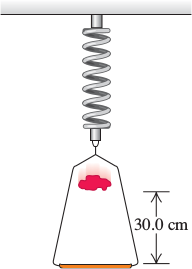
\includegraphics[width=3cm]{plasticine}
\end{wrapfigure}
Un support de 0,15 kg est suspendu au repos à un ressort. Il déforme ainsi le ressort de 0,05m. On laisse tomber sur le support, d'une hauteur
de 30 cm et avec une vitesse initiale nulle, un morceau de plasticine de 0,2 kg. Après l'impact, la plasticine reste collée au support. 
Calculer le déplacement vertical max du support suite à cette collision.

\vspace{3cm}

\paragraph*{Solution}

Tout d'abord, calculons la constante de raideur du ressort à sa position de repos. Avec $s$ la longueur sur laquelle le ressort est étendu au repos, il vient 
\[\sum F_y = -mg + ks = 0 \iff k=\frac{mg}{s} = \frac{(0.15 \mathrm{kg})(9.8 \mathrm{\frac{m}{s^2}})}{0.05 \mathrm m}= 29.4 \mathrm{\frac{N}{m}}\].

Nous allons maintenant calculer la vitesse à laquelle la plasticine arrive lorsqu'elle "percute" le support. 
On sait que, pour une accélération constante, on a $\displaystyle{v^2=v_0^2 + 2a(y-y_0)}$. Comme $v_0 = 0$ et $y-y_0 = 0.3 \mathrm m$, \[v = \sqrt{2(9.8 \mathrm{\frac{m}{s^2}})(0.3 \mathrm m)} = 2.425 \mathrm{\frac{m}{s}}\]

Par la conservation du momentum, on peut établir $-m_Av_{A1} = -(m_A+m_B)v_2$ et donc 
\[v_2 = \left(\frac{m_A}{m_A+m_B}\right)v_{A1} = \left(\frac{0.2 \mathrm{kg}}{0.35 \mathrm{kg}}\right)(2.425 \mathrm{\frac{m}{s}} = 1.386 \mathrm{\frac{m}{s}}\]

Soit $d$ le déplacement entre le point de collision et l'étirement maximum, appliquons le principe de conservation de l'énergie mécanique au système \[K_1 + U_1 + W_{other} = K_2 + U_2\]

\begin{itemize}
	\item $K_1 = \frac{1}{2} mv_1^2 = 0.5(0.350)(1.386)^2 = 0.3362 \mathrm{J}$
	\item $U_1 = 0.5 kx_1^2+mgy_1 = 0.5(29.4)(0.05)^2 + (0.35)(9.8)d = \left(0.03675 + (3.43)d\right) \mathrm{J}$
	\item $U_2 = 0.5(29.4)(0.05+d)^2 = \left(0.03675 + 1.47d+14.7d^2\right) \mathrm{J} $
\end{itemize}

Ce qui nous donne, en isolant d
\[\boxed{d = 0.2319 \mathrm m}\]

\newpage

\paragraph{Question 4}
Définissez le concept de \textit{vitesse terminale} d'un corps en chute libre dans l'air (un parachutiste, par exemple) et déduisez à partir des
lois de la physique adéquates une formule permettant de calculer cette vitesse.

\vspace{3cm}

\paragraph*{Solution}

Lorsqu'un corps est en chute libre dans l'air, il est soumis à 2 forces principales: son poids et la résistance de l'air. Il est donc attiré par la Terre par une force poids d'intensité $w = mg$ et la force opposée à celle induite par le champ gravitationnel est une force d'intensité $f = Dv^2$ où $v$ représente l'intensité du vecteur vitesse dirigé vers le bas et $D$ est une constante liée à la forme du corps et à la viscusité du fluide pénétré (ici, l'air). On voit donc que cette force est proportionnelle au carré de la vitesse. Or, soumis à une accélération vers le bas, cette vitesse augmente sans cesse jusqu'à ce que la la force de résistance de l'air soit égale en intensité à celle de la gravité. Le corps en chute libre atteint donc une vitesse dès lors constante, sa \textbf{vitesse terminale}, dont on peut déduire l'intensité car le corps est alors en \textit{MRU} et on sait, par la première loi de Newton que $\displaystyle{\sum \vec{F} = 0}$ en \textit{MRU}.

On a donc 
$$
	Dv_t^2  =  mg \Longleftrightarrow
	v_t  =  \sqrt{\frac{mg}{D}}
$$

où $v_t$ est représente l'intensité de la vitesse terminale.

\begin{figure}[!h]
	\centering
	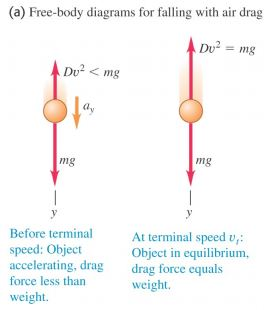
\includegraphics[scale=0.5]{terspeed}
	\caption{FBD du corps en chute libre}
\end{figure}

\end{document}

